\documentclass{beamer}
%\usetheme{Warsaw}
%\usetheme{Madrid}
\usetheme{Marburg}
\usecolortheme{albatross}
\color{yellow}
\setbeamercovered{transparent}
\usepackage{listings}
\usepackage[english]{babel}
\usepackage{color}
\usepackage{caption}
\captionsetup[figure]{labelformat=empty}
\lstset{
%	basicstyle=\footnotesize\ttfamily,
	basicstyle=\tiny\color{white}\ttfamily,
	frame=single,
	extendedchars=true,
	escapechar={@},
}


% Title page details
\title{Qubes OS Documentation Localization}
\subtitle{Past, Present, Future}
\author{m, Tobias Killer}
\institute{}
\date{September 10, 2022}

\begin{document}

\begin{frame}
	\titlepage
\end{frame}

%\begin{frame}
%	\frametitle{Frames und Slides}
%	\framesubtitle{Frames}
%	\begin{itemize}
%		\item<1> erster Punkt
%		\item<2> zweiter Punkt
%		\item<3> dritter Punkt
%	\end{itemize}
%	\begin{block}{Ein Standardblock}
%	\end{block}
%	\begin{exampleblock}{Ein Beispielblock}
%	\end{exampleblock}
%	\begin{alertblock}{Ein Alarmblock}
%	\end{alertblock}
%\end{frame}

\AtBeginSection[]
{
\begin{frame}<beamer>
\frametitle{Outline}
\tableofcontents[currentsection]
\end{frame}
}

\begin{frame}
	\frametitle{Outline}
	\tableofcontents
\end{frame}

\section{Introduction \& Welcome}

\begin{frame}
	\frametitle{Introduction}
	\begin{itemize}
		\item Goal: continuous reliable localization of the Qubes OS documentation
		\item Translation (tl8n)
		\begin{itemize}
			\item transferring the meaning of a text from one language into another
		\end{itemize}
		\item Internationalization (i18n)
		\begin{itemize}
			\item making everything flexible and ready for localization
		\end{itemize}
		\item Localization (l10n)
		\begin{itemize}
			\item translation into a concrete language \& cultural context (restroom vs bathroom)
		\end{itemize}
	\end{itemize}
\end{frame}

\section{Official Qubes OS Documentation}

\begin{frame}
	\frametitle{Official Qubes OS Documentation}
	\begin{itemize}
		\item Several Git repositories
		\begin{itemize}
				\item qubesos.github.io (core pages)
				\item qubes-doc (documentation pages)
				\item qubes-hcl (Hardware Compatibility List data files)
				\item qubes-posts
				\item qubes-attachment
		\end{itemize}
		\item Github Pages + Jekyll + Liquid Template Language + Source Files = static website

		
	\end{itemize}
\end{frame}


\begin{frame}
	\frametitle{Challenges}
	\begin{itemize}
		\item Community effort
		\item Security first
		\begin{itemize}
			\item avoid unknown third-party plugins
			\item distrust translations
		\end{itemize}
	\end{itemize}
\end{frame}

\begin{frame}
	\frametitle{Challenges (2)}
	\begin{itemize}
		\item Internationalization
		\begin{itemize}
			\item difficult due to a continuously changing website
			\item also vice versa
		\end{itemize}
		\item Markdown files
		\begin{itemize}
			\item YAML front matter
			\item internal links
			\begin{itemize}
				\item anchors included
			\end{itemize}
		\end{itemize}
	\end{itemize}
\end{frame}

\begin{frame}
	\frametitle{Challenges (3)}
	\begin{itemize}
		\item URLs
		\begin{exampleblock}{How to localize this link?}
		\scriptsize{https://www.qubes-os.org/doc/system-requirements/\#recommended}
	\end{exampleblock}
		\item Lack of a language switcher
	\end{itemize}
\end{frame}

\section{What have we done so far? The past}

\begin{frame}
	\frametitle{What have we done so far? The past}
	\begin{itemize}
		\item Transifex
		\begin{itemize}
			\item web platform for projects and translators making localization
			\item line-by-line translation and review
			\begin{itemize}
				\item Markdown convention: one sentence per line (not enforceable)
			\end{itemize}
			\item scriptable upload and download
		\end{itemize}
	\end{itemize}
\end{frame}

\begin{frame}
	\frametitle{What have we done so far? The past (2)}
		\begin{itemize}
			\item Plain text files uploaded to Transifex
	\end{itemize}
\end{frame}

\begin{frame}
	\frametitle{What have we done so far? The past (3)}
	\begin{itemize}
		\item i18n: Markdown files indexable for different languages
%\begin{verbatim}
%---
%lang: en
%layout: doc
%permalink: /doc/how-to-copy-and-paste-text/
%redirect_from:
%- /doc/copy-paste/
%- /en/doc/copy-paste/
%- /doc/CopyPaste/
%- /wiki/CopyPaste/
%ref: 196
%title: How to copy and paste text
%---
%\end{verbatim}
\begin{exampleblock}{qubes-doc/user/how-to-guides/how-to-copy-and-paste-text.md}
\texttt{$-$$-$$-$\\
\alert{lang: en}\\
layout: doc\\
permalink: /doc/how-to-copy-and-paste-text/\\
redirect\_from:\\
$-$ /doc/copy-paste/\\
$-$ /en/doc/copy-paste/\\
$-$ /doc/CopyPaste/\\
$-$ /wiki/CopyPaste/\\
\alert{ref: 196}\\
title: How to copy and paste text\\
$-$$-$$-$}
\end{exampleblock}
	\end{itemize}
\end{frame}

\begin{frame}
	\frametitle{What have we done so far? The past (4)}
	\begin{itemize}
		\item i18n: HTML  files indexable for different localizations
		\begin{exampleblock}{qubesos.github.io/\_includes/head.html}
%\begin{verbatim}
%<!-- Localization -->
%
%  
%
%  
%
%
%  
%    
%  
%    
%
%<html lang="{{ pagelang }}" dir="{{ textdir }}">
%\end{verbatim}
\texttt{$<$!$-$$-$ Localization $-$$-$$>$\\
\{\% if \alert{page.lang} \%\}\\
\ \ \{\% assign \alert{pagelang} = \alert{page.lang} \%\}\\
\{\% else \%\}\\
\ \ \{\% assign pagelang = "en" \%\}\\
\{\% endif \%\}\\
\{\% case pagelang \%\}\\
\ \ \{\% when "ar", "arc", "dv", "fa", "ha", "he", […] \%\}\\
\ \ \ \ \{\% assign textdir = "rtl" \%\}\\
\ \ \{\% else \%\}\\
\ \ \ \ \{\% assign textdir = "ltr" \%\}\\
\{\% endcase \%\}\\
$<$html lang="\{\{ \alert{pagelang} \}\}" dir="\{\{ textdir \}\}"$>$}
\end{exampleblock}
	\end{itemize}
\end{frame}

\begin{frame}
	\frametitle{What have we done so far? The past (5)}
	\begin{itemize}
		\item How to make localization comfortable, easy and error-unprone for translators?
		\begin{itemize}
			\item automatic internal link localization
			\item automatic insertion of unlocalized anchors into localized files (no localization of anchors needed)
		\end{itemize}
		\item URL example for German
		\begin{exampleblock}{How to localize this link?}
			\scriptsize{https://www.qubes-os.org\alert{/de}/doc/system-requirements/\#recommended}
		\end{exampleblock}
	\end{itemize}
\end{frame}

\begin{frame}
	\frametitle{What have we done so far? The past (6)}
	\begin{itemize}
		\item A dedicated mailing list (qubes-translation)
		\item A homemade language switcher
		\item Python, Bash and Ruby scripts
		\item A comprehensive set of rules for translators/reviewers
	\end{itemize}
\end{frame}





\section{Where are we? The present}

\begin{frame}
	\frametitle{Read The Docs community}
	\begin{itemize}
		\item Pros and Cons
		\item Conversion from Markdown to ReStructuredText (RST)
		\item Local development
		\item Transifex workflow
		\item Deployment
		\item Revisited Qubes OS website contents
	\end{itemize}
\end{frame}


\begin{frame}
	\frametitle{Read The Docs 4 Qubes doc - pros and cons}
	\begin{itemize}
		\item Pros
		\begin{itemize}
			\item Versioning $\rightarrow$  release specific documentation
			\item Sphinx inherited goodies: 
			\begin{itemize}
				\item internationalization \& localization support out of the box, PDF \& EPUB generation, easy local development environment 
			\end{itemize}
			\item Continuous documentation deployment
			\item 1 CVE  \tiny{\footnote{\tiny{https://www.cvedetails.com/vendor/20051/Readthedocs.html}}}
		\end{itemize}
		\item Cons 
		\begin{itemize}
			\item Different designs
			\item Two different tech stacks for website \& documentatoin
			\item Getting familiar with a new markup language
			\item Minor buggy deployment issues
			\item Advertising \& analytics \tiny{\footnote{\tiny{https://docs.readthedocs.io/en/latest/advertising/advertising-details.html\#analytics}}}
		\end{itemize}
		
	\end{itemize}
\end{frame}


\begin{frame}[fragile]
	\frametitle{Read The Docs - MD2RST }
	\begin{itemize}
		\item Support for Markdown via MkDocs generator, localization not supported \tiny{\footnote{\tiny{https://docs.readthedocs.io/en/stable/localization.html}}}
		\large{\item Support of RST via sphinx generator} \tiny{\footnote{\tiny{https://www.sphinx-doc.org/en/master/}}}
		
		\tiny{
		\large{\item Using pandoc}
		\begin{exampleblock}{pandoc}
			\begin{lstlisting}[language=bash]
$ pandoc doc.md --from markdown --to rst -s -o doc.rst
			\end{lstlisting}
		\end{exampleblock}
		}
		
		\large{\item Scripted pypandoc \& post-processing}
		\begin{itemize}
			\item cross-referencing using sphinx \textbf{:doc:} and \textbf{:ref:} roles
			\item further handling of Jekyll specific permalinks
				\tiny{
					\begin{exampleblock}{md2rst}
					\begin{lstlisting}[language=bash]
$ python md2rst.py --config config.toml
					\end{lstlisting}
			\end{exampleblock}
				}
		\end{itemize}
		\item Run only once, fix errors \& deploy 
		
	\end{itemize}
\end{frame}



\begin{frame}[fragile]
	\frametitle{Read The Docs - local development }
%	\begin{itemize}
%		\item Easy as in
%		\begin{lstlisting}[language=Python]
		\begin{exampleblock}{render locally}
		\begin{lstlisting}[language=bash]
$ sphinx-view . -c conf.py
		\end{lstlisting}
		\end{exampleblock}
	
		\begin{exampleblock}{conf.py}
		\tiny{
		\begin{lstlisting}[language=python]
...

html_static_path = ['attachment/doc']
extensions = ['sphinx.ext.autosectionlabel']
autosectionlabel_prefix_document = True
source_suffix = {'.rst': 'restructuredtext'}
templates_path = ['_templates']
root_doc = "index"
exclude_patterns = ['_dev/*','attachment/*','**/*.txt']
html_theme = 'default'		
epub_show_urls = 'footnote'
latex_show_urls ='footnote'

...	
		\end{lstlisting}
		}
		\end{exampleblock}
		
%	\end{itemize}
\end{frame}



\begin{frame}[fragile]
	\frametitle{Read The Docs - sphinx build log }
		\begin{exampleblock}{running sphinx v4.5.0 ...}
\tiny{
		\begin{lstlisting}
WARNING: Pygments lexer name 'shell_session' is not known
WARNING: undefined label:
WARNING: unknown document
WARNING: document isn't included in any toctree
WARNING: Inline literal start-string without end-string.
WARNING: Block quote ends without a blank line; unexpected unindent.
WARNING: Title underline too short.
ERROR: Unexpected indentation.
ERROR: Error in "figure" directive:
		\end{lstlisting}
	}
\end{exampleblock}	

	\begin{exampleblock}{linkcheck}
\tiny{
	\begin{lstlisting}[language=bash]
$ sphinx-build -b linkcheck . _build/linkcheck
	\end{lstlisting}
}
Output: $build/linkcheck/output.(json|txt)$
\end{exampleblock}

\end{frame}

\begin{frame}[fragile]
	\frametitle{Read The Docs - Transifex workflow}
%	\begin{itemize}
%		\item conf.py
		\begin{exampleblock}{conf.py}
	\tiny{
		\begin{lstlisting}[language=python]
...

gettext_uuid=True
gettext_compact=False	
locale_dirs = ['_translated']	

...	
		\end{lstlisting}
	}
\end{exampleblock}

	\begin{exampleblock}{sphinx localization}
	\tiny{
		\begin{lstlisting}[language=bash]
$ sphinx-build -b gettext . _build/gettext
		\end{lstlisting}
	}
\end{exampleblock}

\end{frame}


\begin{frame}[fragile]
	\frametitle{Read The Docs - scripted Transifex workflow }
%		\begin{itemize}
%			\item Old tx client (extinct in Nov 2022)
		\begin{exampleblock}{initial configuration}
			\tiny{
				\begin{lstlisting}[language=bash]
$ tx init --token 1/XXX --no-interactive;
$ mkdir _translated; (defined in conf.py as locale_dir )
				\end{lstlisting}
			}
		\end{exampleblock}
	
			\begin{exampleblock}{create translatable files}
		\tiny{
			\begin{lstlisting}[language=bash]
$ sphinx-build -b gettext . _translated/_build/gettext;
			\end{lstlisting}
		}
	\end{exampleblock}

			\begin{exampleblock}{transifex mapping, push \& pull}
	\tiny{
		\begin{lstlisting}[language=bash]
$ tx config mapping-bulk --project  qubes --file-extension '.pot' \
--source-file-dir _translated/_build/gettext/ \
--source-lang en --type PO \
--expression '_translated/<lang>/LC_MESSAGES/{filepath}/{filename}.po' \
--execute;
$ tx push --source;
		\end{lstlisting}
	}
\end{exampleblock}
			\begin{exampleblock}{local build}
	\tiny{
		\begin{lstlisting}[language=bash]
$ tx pull -l de;
$ sphinx-build -b html -D language=de . _translated/_build/html/de -v -a;
		\end{lstlisting}
	}
\end{exampleblock}

%		\end{itemize}
	\end{frame}



\begin{frame}[fragile]
	\frametitle{Read The Docs - deployment }
		\begin{exampleblock}{.readthedocs.yaml}
			\tiny{
				\begin{lstlisting}[language=bash]
version: 2

build:
 os: "ubuntu-22.04"
 tools:
  python: "3.10"
	  
sphinx:
 builder: html
 configuration: conf.py
 fail_on_warning: false
	
python:
 install:
  - requirements: requirements.txt
	  
formats:
 - pdf
 - epub
				\end{lstlisting}
			}
			
		\end{exampleblock}
%	\end{itemize}
\end{frame}


\begin{frame}
	\frametitle{What do we have till now?}
	
	\begin{columns}[c]
		
		% create the column with the first image, that occupies
		% half of the slide
		\begin{column}{.5\textwidth}
			\begin{figure}
				\centering
				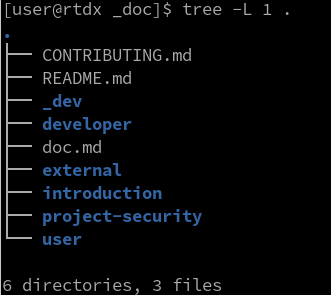
\includegraphics[scale=0.45]{pix/status-a.png}
				\caption{\tiny{1. Original \textbf{qubes-doc} repo Markdown contents}}
			\end{figure}      
		\end{column}
		
		% create the column with the second image, that also
		% occupies half of the slide
		\begin{column}{.5\textwidth}
			\begin{figure}
				\centering
				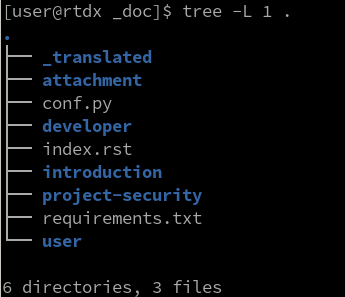
\includegraphics[scale=0.45]{pix/status-b.png}
				\caption{\tiny{2a. Converted \textbf{qubes-doc} repo RST contents}}
			\end{figure}
		\end{column}
		
	\end{columns}
	\begin{figure}
		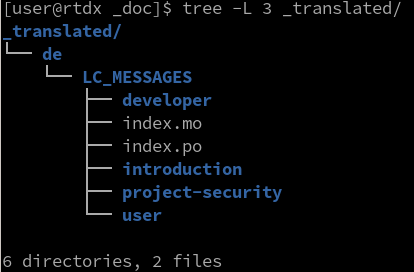
\includegraphics[scale=0.45]{pix/status-c.png}
		\caption{\tiny{2b. Localized content downloaded from Transifex}}
	\end{figure}
	
\end{frame}

\begin{frame}
	\frametitle{Read The Docs - translation management }
	\begin{enumerate}
		\item (A) Import qubes-rst-doc project with English as default language
		\item (B) Manually import the same qubes-rst-doc repo containing the pulled translations from Transifex with Non-English as default language
	\end{enumerate}
	\begin{figure}
		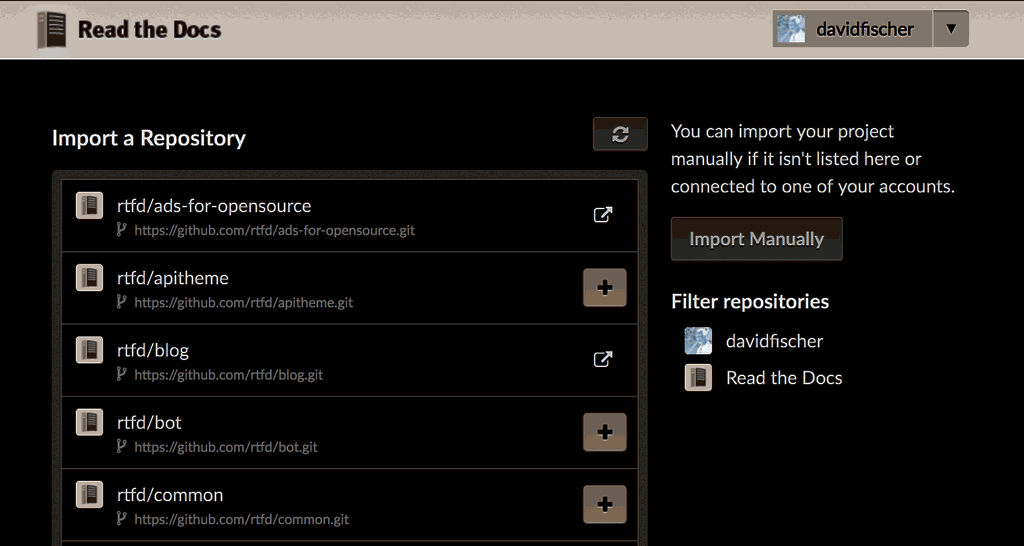
\includegraphics[scale=0.15]{pix/import-a-repository.png}
		\caption{Source \footnote{https://docs.readthedocs.io/en/stable/intro/import-guide.html}}
		\label{fig:rtd-import}
	\end{figure}
	
\end{frame}


\begin{frame}[fragile]
	\frametitle{Read The Docs - translation management }
	\begin{enumerate}
		\setcounter{enumi}{2}
		\item In (A) add the new manually imported repo (B) as a translation 
		\item Enjoy
	\end{enumerate}
	\begin{figure}
		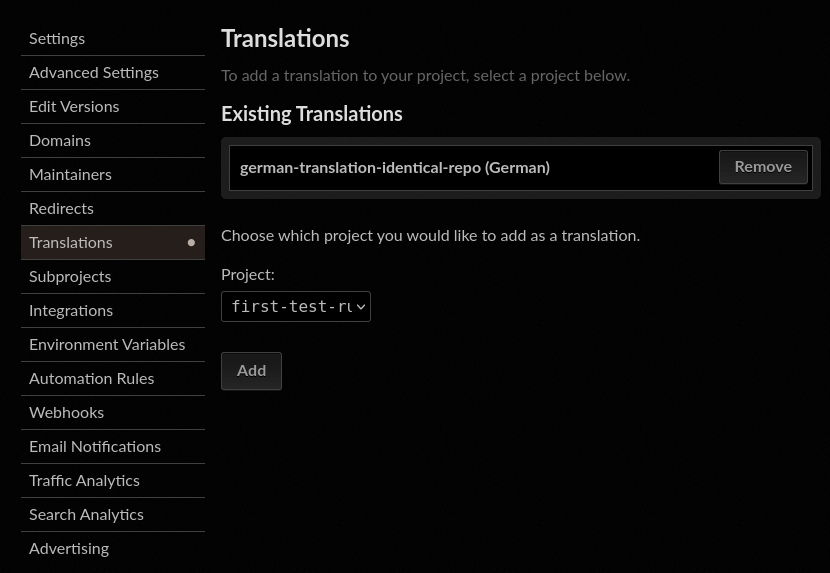
\includegraphics[scale=0.15]{pix/translation-rtd.png}
		\label{fig:rtd-r}
	\end{figure}
\end{frame}

\begin{frame}
	\frametitle{Read The Docs - current status \tiny{\footnote{\tiny{https://current-qubes-docrtd.readthedocs.io/en/latest/}}}}
	\begin{figure}
		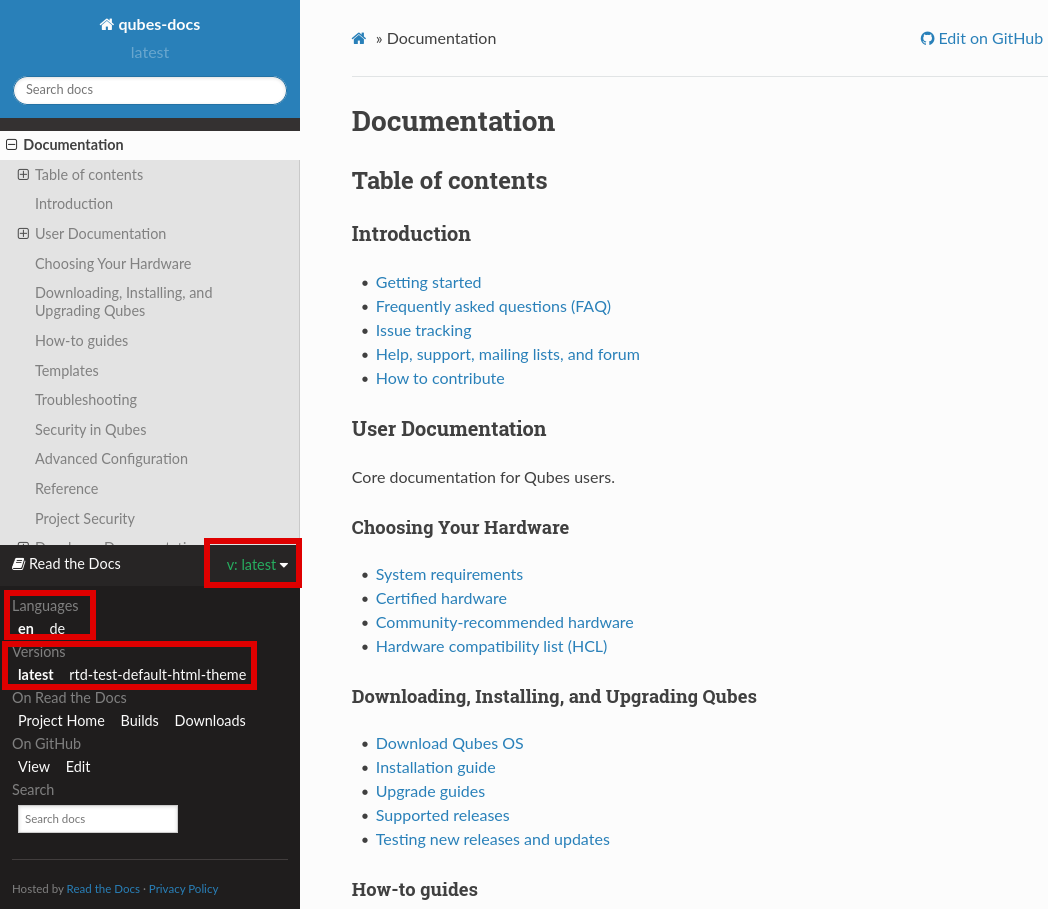
\includegraphics[scale=0.25]{pix/rtd-1.png}
		\label{fig:rtd-1}
	\end{figure}
\end{frame}

\begin{frame}
	\frametitle{Read The Docs - current status \tiny{\footnote{\tiny{https://current-qubes-docrtd.readthedocs.io/de/latest/}}}}
	\begin{figure}
		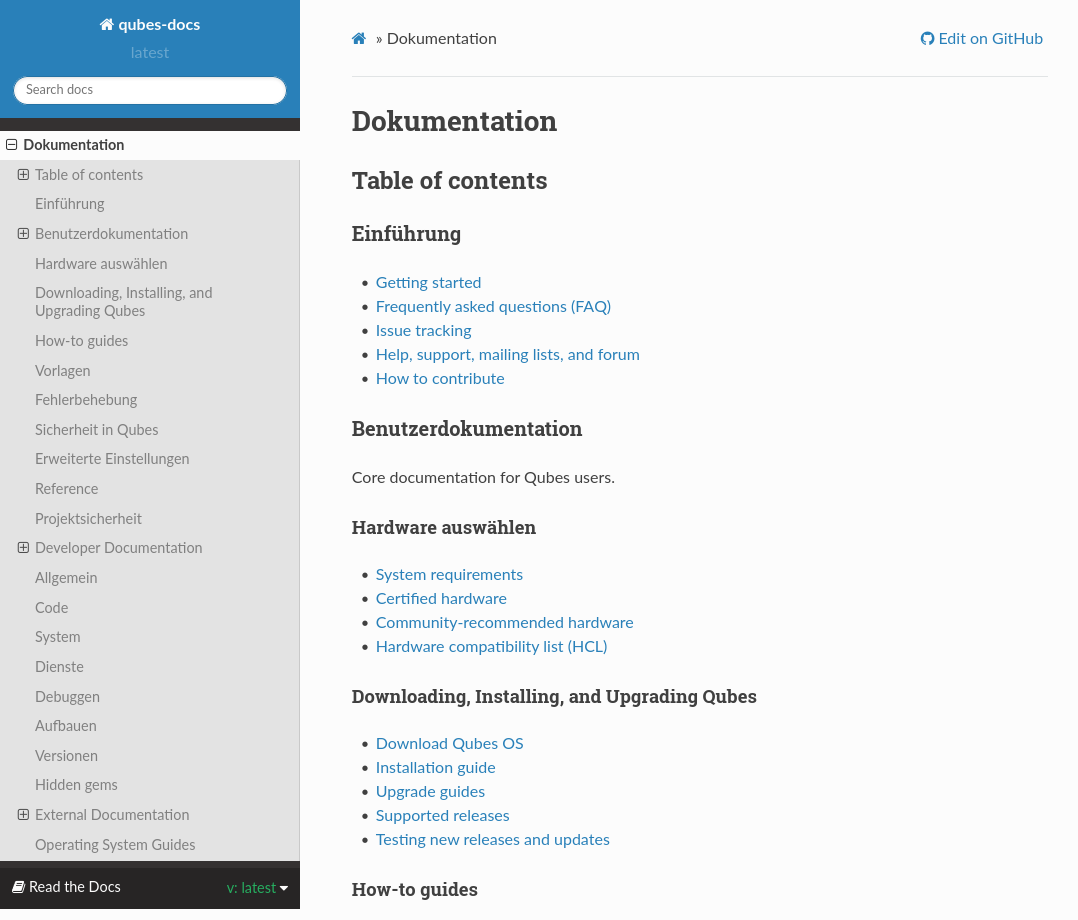
\includegraphics[scale=0.25]{pix/rtd-2.png}
		\label{fig:rtd-2}
	\end{figure}
\end{frame}



\begin{frame}
	\frametitle{Continuous localization of the official Qubes OS documentation}
	\framesubtitle{As RestructredText on ReadTheDocs}
	\begin{itemize}
		\item Old vs new transifex client (OR)
		 Use Transifex Integration App \tiny{\footnote{\tiny{https://github.com/apps/transifex-integration}}} \large{(not tested)}
		\large{\begin{itemize}
				\item Transifex authentication on Github
				\item Github repository to Transifex project
				\item files \& automated action selection
		\end{itemize}}			
		\item Build \& deploy documentation on every commit on RtD
	\end{itemize}
	
\end{frame}


\begin{frame}
	\frametitle{Read The Docs - nice to haves atm}
	\begin{enumerate}
		\item Liquid vs Jinja Templating
		\item Sphinx-reredirects extension
	\end{enumerate}
\end{frame}


\begin{frame}
	\frametitle{Localization of the official Qubes OS documentation}
	\framesubtitle{As part of the official Qubes OS Website as with Markdown}
	%	\begin{figure}
		%		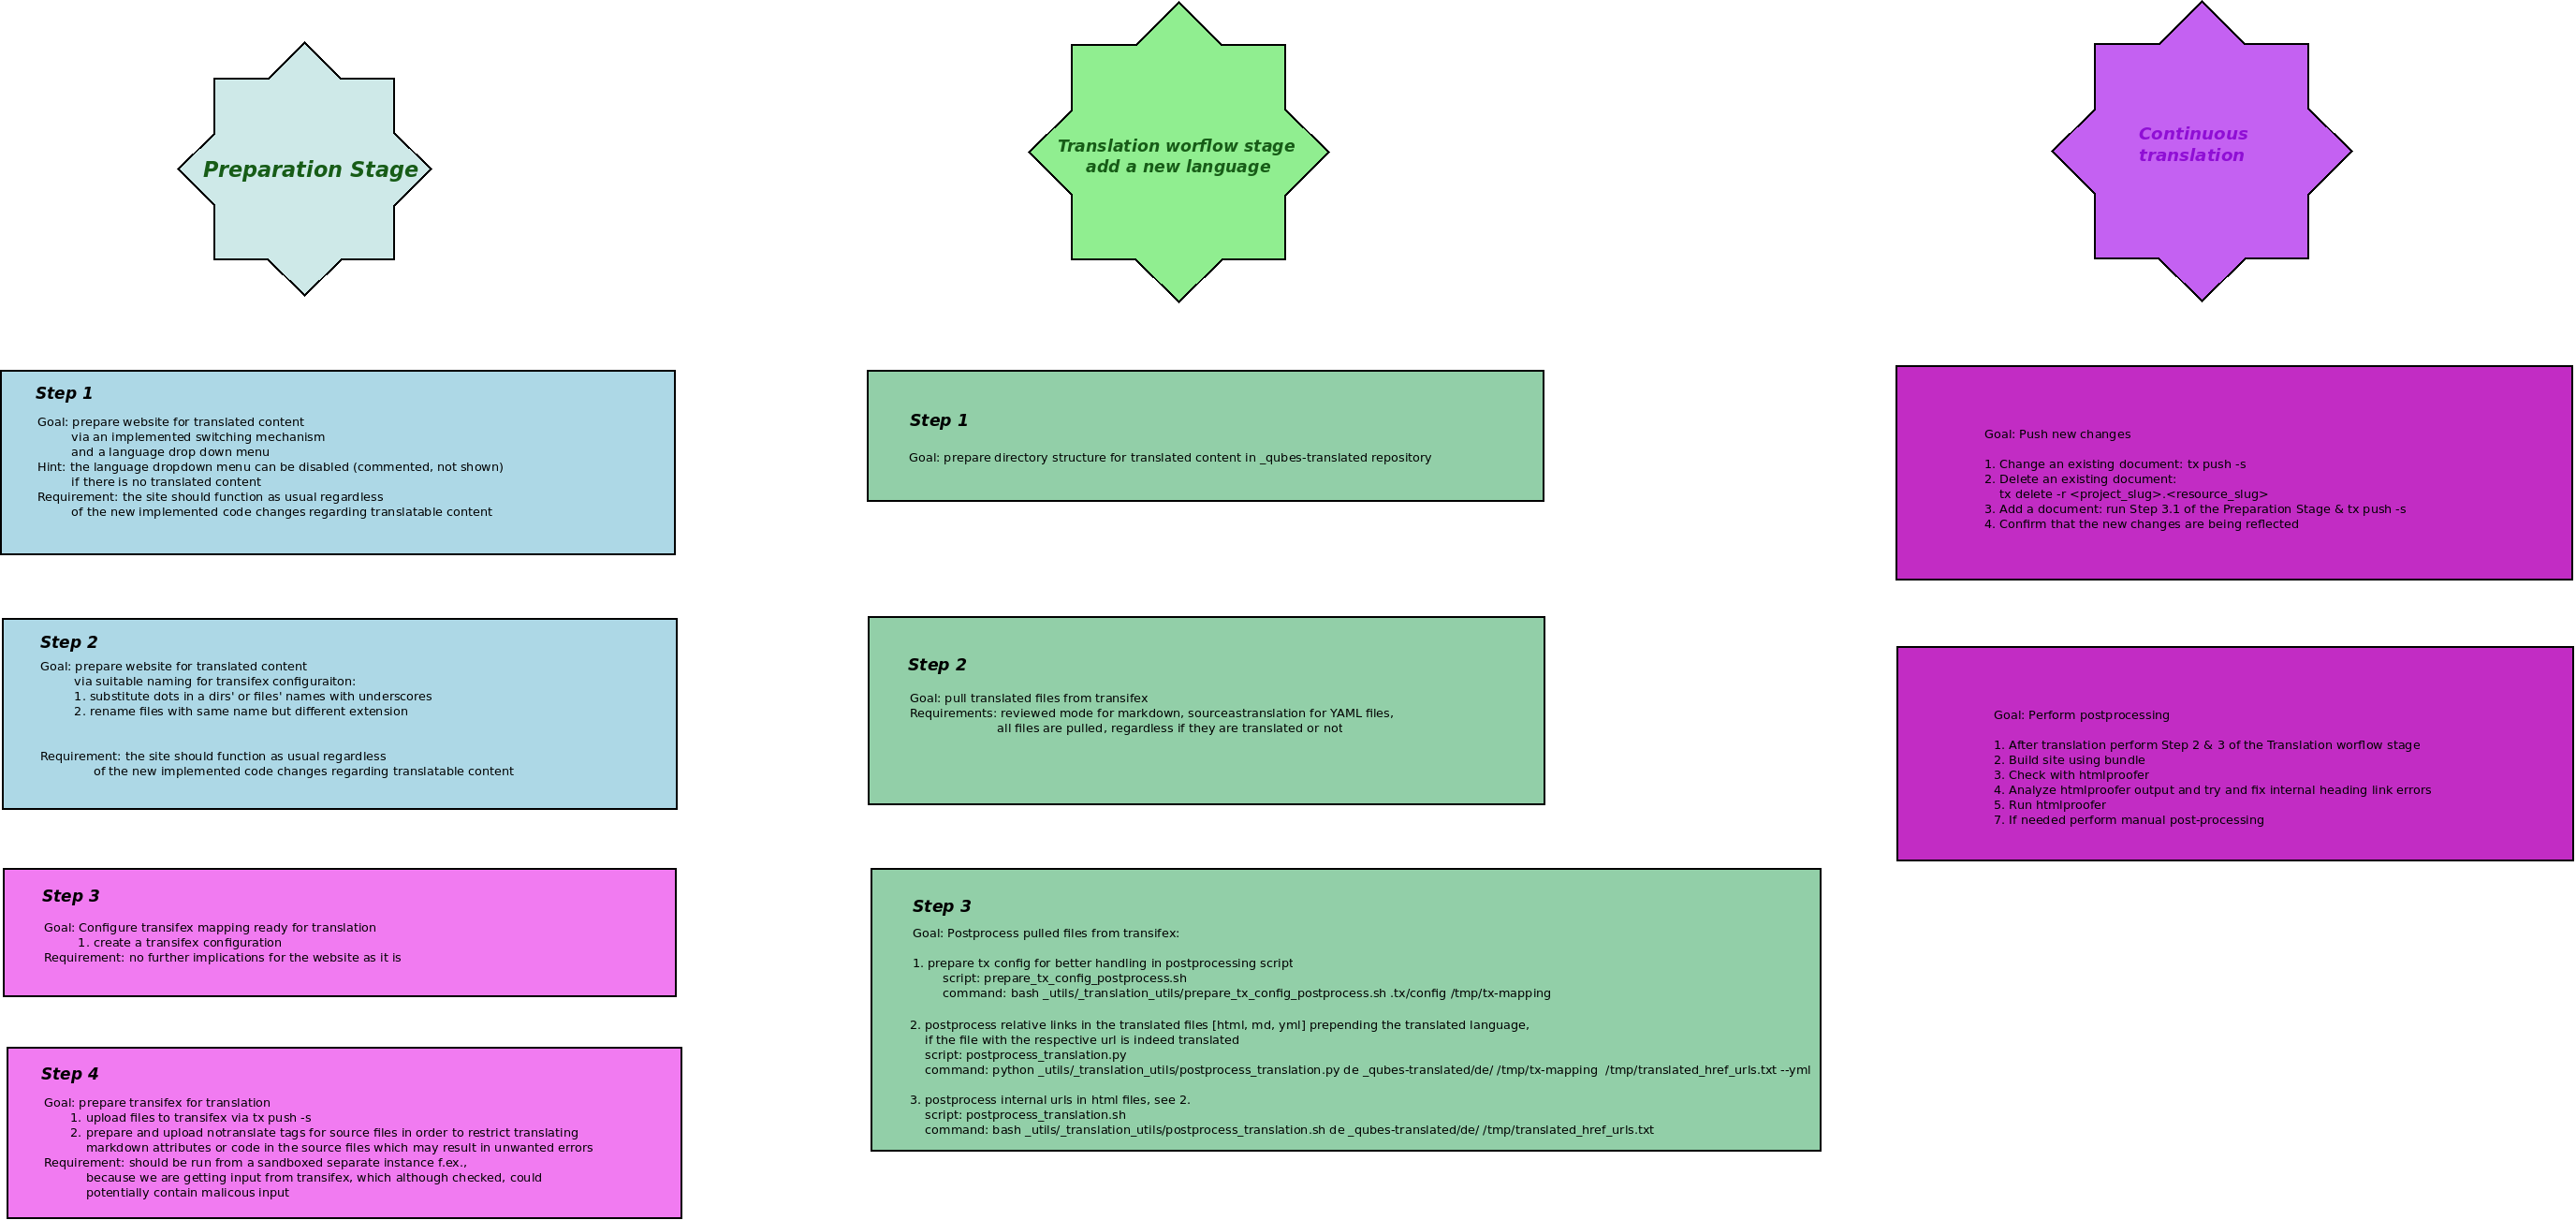
\includegraphics[width=\linewidth]{pix/mdworkflow.png}
		%		\caption{Localization of the official Qubes OS documentation workflow}
		%		\label{fig:mdworkflow}
		%	\end{figure}
	\begin{enumerate}
		\item Prepare, create tx configuration and push
		\item Pull and post-process translations (OR)
		Use Transifex Integration App and post-process translations	
		\item Build \& deploy documentation 
	\end{enumerate}
	\bigskip
	\begin{itemize}
		\item Post-processing step after pulling translations (°\`\_´°)		
		\item Still a viable way forward
		\item Can be used for localization of the website
	\end{itemize}
\end{frame}

\section{Quo vadis? The future}

\begin{frame}
	\frametitle{Looking forward}
	\begin{enumerate}
		\item Official decision - RtD/RST or github-pages/Markdown?
		\item Testing and fixing bugs phase
		\item Qubes OS documentation hosted on RTD/github-pages
		\item Transifex translation
		\item Localized documentation hosted on RTD/github-pages
		\item Qubes OS official website localization (pages, perhaps even posts)
		\item Community documentation localization
	\end{enumerate}
\end{frame}

\begin{frame}
	\frametitle{Specific tasks (sample)}
	\begin{itemize}
		\item ReStructuredText documentation guide
		\item Localization FAQ, glossary \& guidelines
		\item Create github issue label/project localization
		\item Create localization issue template
		\item Create language specific documentation file inside the qubes-translation submodule for the specific language to be maintained by translators as a README.md Refer to it from the general language specific guidelines
		\item Update the general contribution guidelines
		\item Create a localization brief
		\item Clean up the qubes os transifex project vocabularies
		\item Create tutorial vids for translating/maintaining
		
	\end{itemize}
\end{frame}


\begin{frame}
	\frametitle{We need you!}
	\begin{center}
		Get in touch! 
		\bigskip
		Reach out via the translation mailing list \textbf{qubes-translation@googlegroups.com}
	\end{center}
\end{frame}



\begin{frame}
	\frametitle{Thank you!}
	\begin{center}
		Discussion, questions, suggestions, critique are welcome!
	\end{center}
\end{frame}

\end{document}

